\section{Adiabatic Logic}
\label{sec:adiabatic}

\subsection{notes}

\begin{itemize}

\item{Pros:}

\begin{itemize}

\item{exponential power saving}

\end{itemize}

\end{itemize}

\subsection{Design}
As discussed in section \ref{sec:intro}, energy is lost as the transistors in a circuit change state.
Adiabatic logic attempts to counter this by slowly charging up the components, preventing there ever being a continuous channel from the supply rail to ground.
As such the heat dissipation lost during switching is drastically minimised.
Clearly this has the effect of heavily restricting the maximum speed at which the circuit can operate.

The effect of this can be seen in figure \ref{fig:convvsadia}.
When the conventional CMOS logic input voltage rises suddenly there is an observable peak in the voltage across the resistance.
This high voltage causes a large current flow and hence a large heat dissipation in the resistance.
The current through the resistance causes the capacitor to charge, reducing the voltage across the resistor and preventing further power loss.
In the adiabatic setup, the slower change in the input results in the capacitor being able to keep up with the increase in potential with a minimal current through the resistor, hence significantly less power is dissipated.

\begin{figure}
	\centering
	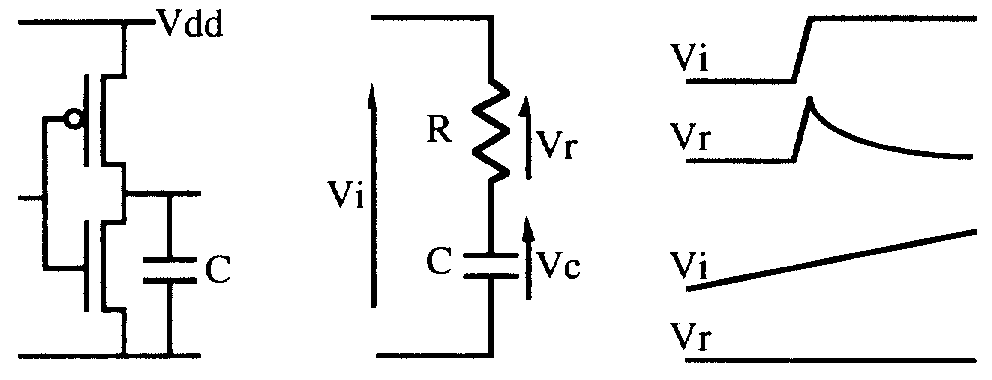
\includegraphics[width=\columnwidth]{../../images/conv_vs_adiabatic.png}
	\caption{Conventional CMOS vs. Adiabatic CMOS in terms of power consumption, shown through the use of the equivalent circuit \cite{DynAdiabatic}}
	\label{fig:convvsadia}
\end{figure}

In order to achieve the energy saving, adiabatic logic uses a number of stages to set itself up.
Firstly the circuit passes through a \emph{precharge} stage.
In this stage the nodes in the circuit are preloaded with a charge.
Secondly comes the \emph{evaluation} stage, during which the logical expression is evaluated, and the various nodes either remain charged or discharge as required.
Then the output can be read from the gate.
This requirement dictates that adiabatic circuits have a complex clocking circuitry, able to provide two different phases.
Creating this complex clock results in a further loss of power, as such the design of this clock must have careful attention paid to it to ensure that it does not restrict the power savings.
Given all of this, adiabatic circuits are able to produce power savings of the order of 10-20 while maintaining speeds in the hundreds of megahertz \cite{PAL, SCAL, DynAdiabatic, TSEL, PALadder}

A by product of the slower switching involved with adiabatic circuits is that switching noise is reduced.
This is a much more critical effect in mixed signal circuits, as opposed to digital only systems, as the analogue circuitry is much more sensitive to noise.
Another advantage of adiabatic logic is its simplicity in production, as in general it requires nothing more than standard CMOS logic gates, with the exception of the clocking circuitry.

In the switching process, a small lump of charge is moved from the power rail to the ground rail during each switching process.
While power is saved from the spike prevention in each switch, this small packet of charge being essentially thrown away is rather wasteful.
As such the use of charge recovery circuitry is advised with adiabatic circuits.
Some adiabatic circuits, such as those discussed in sections \ref{sec:PAL} and \ref{sec:LPAL} include the recovery mechanism as part of the logic.

\subsection{Variations}

\subsubsection{Adiabatic Dynamic Logic}
\label{sec:ADL}
Adiabatic Dynamic Logic as defined by \citeauthor{DynAdiabatic} in \cite{DynAdiabatic} adds two additional stages to the cycle, an \emph{input} stage and a \emph{latch} stage. 
Adiabaticity requires that there is never a large potential across the transistor channel while it is conducting, otherwise the same high switching current would be experienced as in conventional CMOS.
The input and latch stages help to achieve this by providing a time during which the input can change without causing non-adiabatic effects, and by ensuring the output is stable for a measurable amount of time in the latch phase.

\begin{figure}
	\centering
	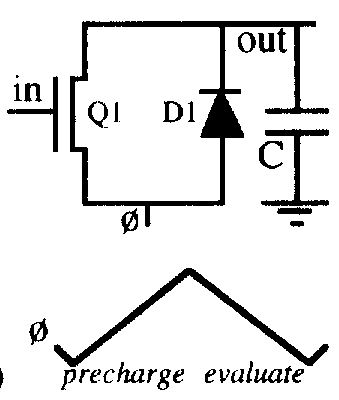
\includegraphics[width=100px]{../../images/ADL.png}
	\caption{Circuit diagram of Adiabatic Dynamic Logic \cite{DynAdiabatic}}
	\label{fig:adl}
\end{figure}

\subsubsection{PAL}
\label{sec:PAL}
Pass-transistor Adiabatic Logic uses a sinusoidal power clock, connected to the nodes through an evaluating NMOS circuit, and also through a single PMOS transistor.
An example of a PAL inverter is shown in figure \ref{fig:pal}.
This inverter circuitry is fairly simple, however more complex functions can be achieved by adding to the NMOS circuitry connecting to the OUT node, and creating a complimentary NMOS function on the /OUT node, as shown in figure \ref{fig:palandor}.

Focussing on the inverter, as the power clock rises from low to high one of the NMOS transistors conducts, allowing the charge to rise on the output node.
The complementary output node will remain low as its respective NMOS does not conduct.
As the charge rises it causes the PMOS transistor to also conduct, allowing the output to reach the peak voltage of the power clock.
When this peak is reached, the output is valid.
As the voltage on the power clock begins to fall away the charge on the output node is discharged to the power clock, resulting in the energy being recovered.

\begin{figure}
	\centering
	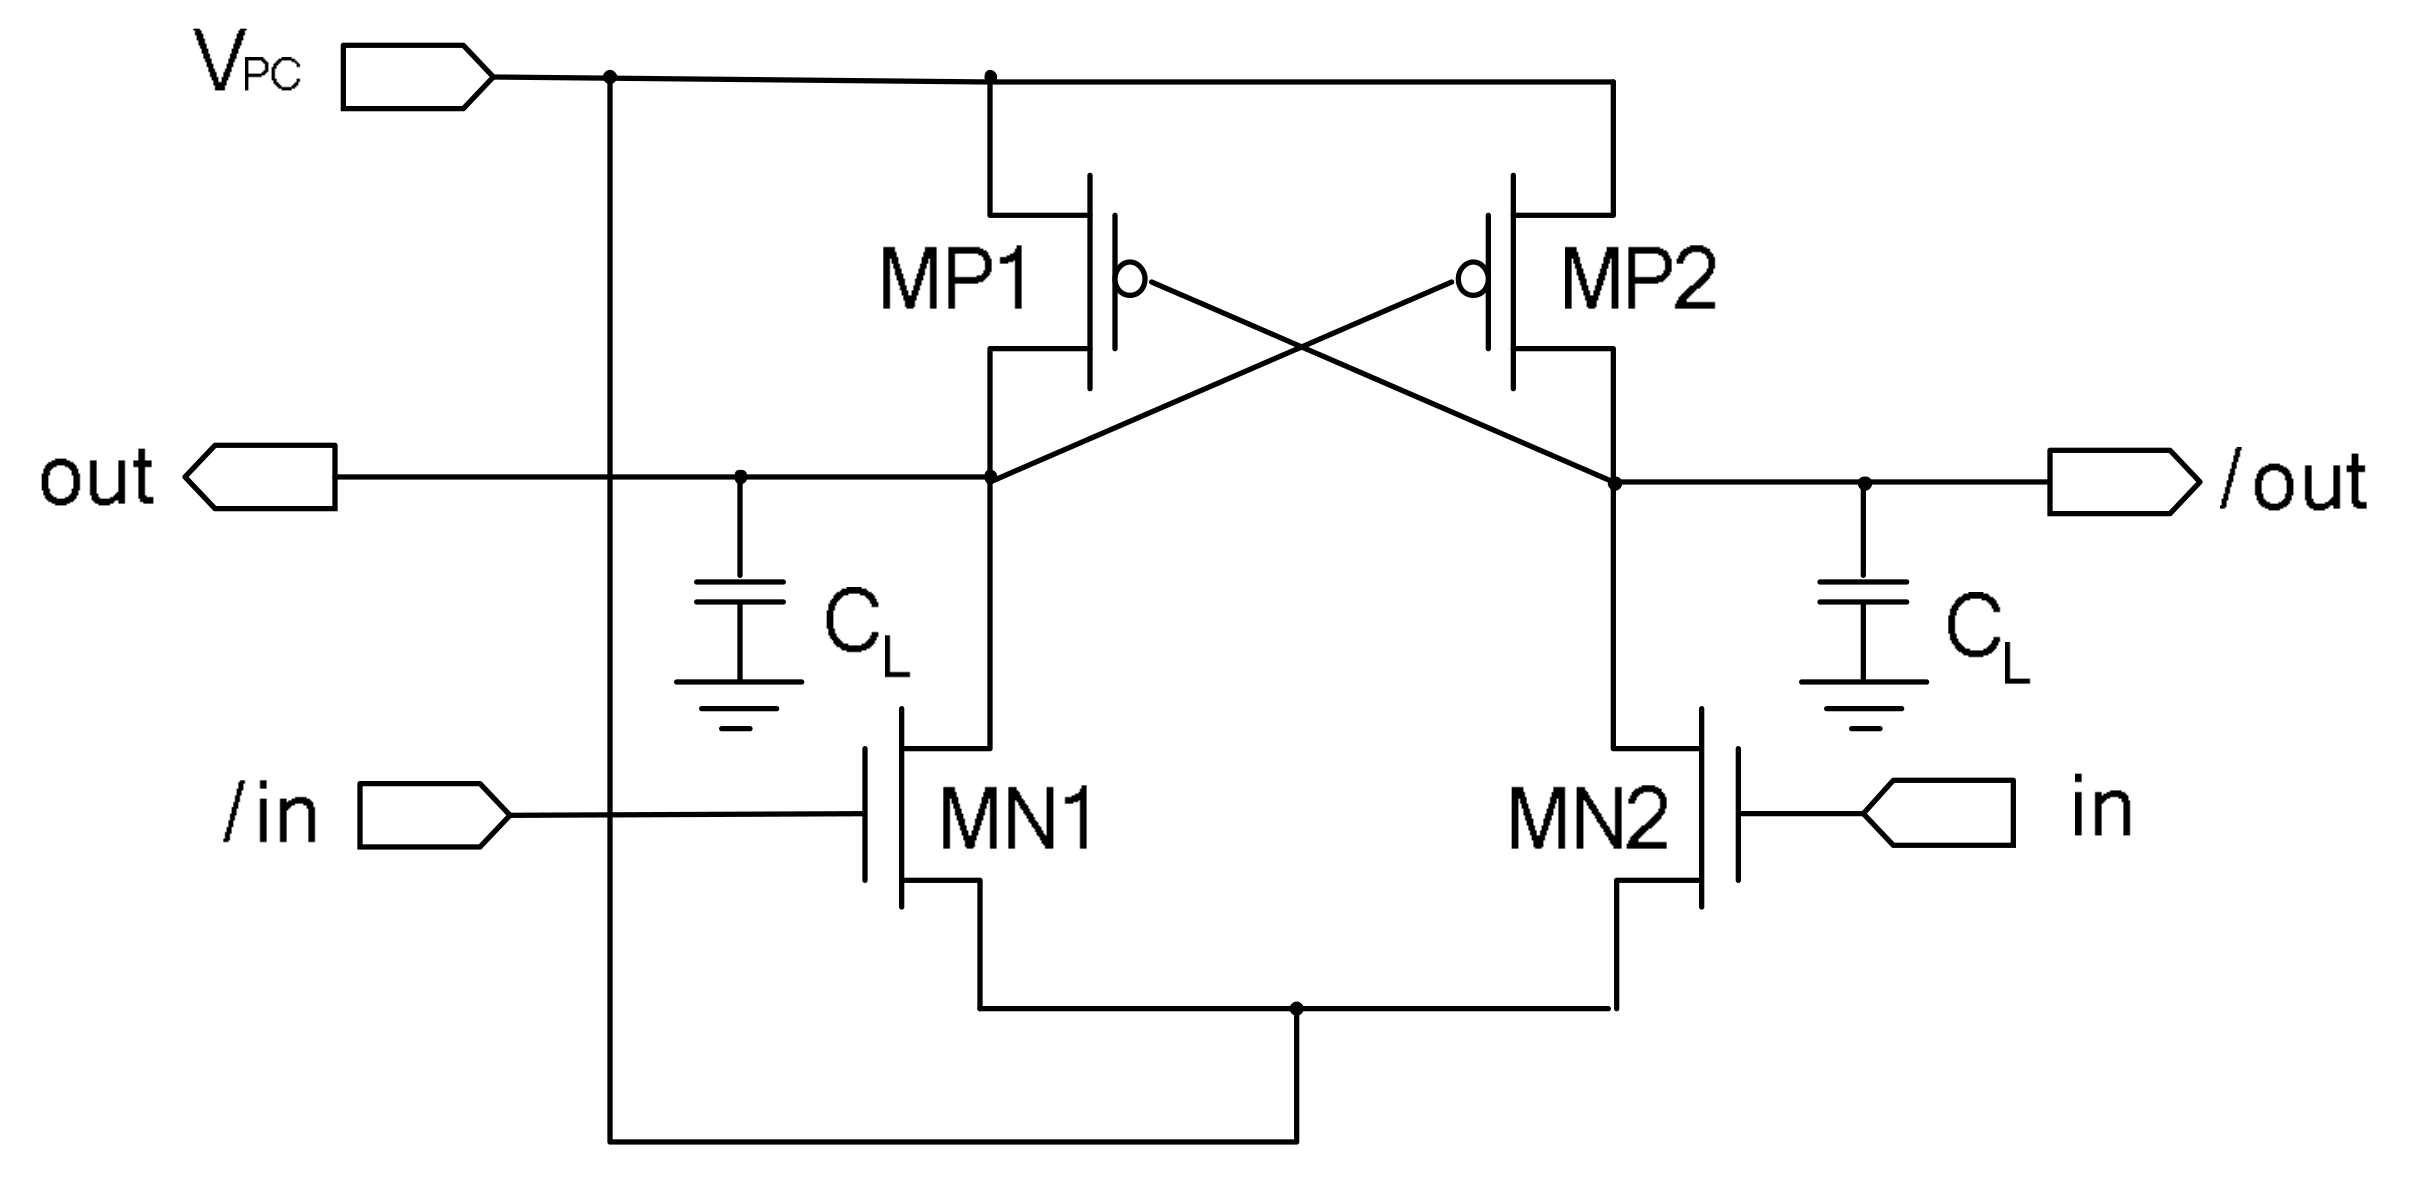
\includegraphics[width=\columnwidth]{../../images/PAL.png}
	\caption{Circuit diagram of a PAL inverter \cite{LPAL}}
	\label{fig:pal}
\end{figure}

A key advantage of PAL over many other adiabatic systems is that it only requires a single clock source \cite{PALsingle, PAL}.
Given this fact it generates savings in the order of 10-20 \cite{PAL} while losing very little power in clock generation.

\begin{figure}
	\centering
	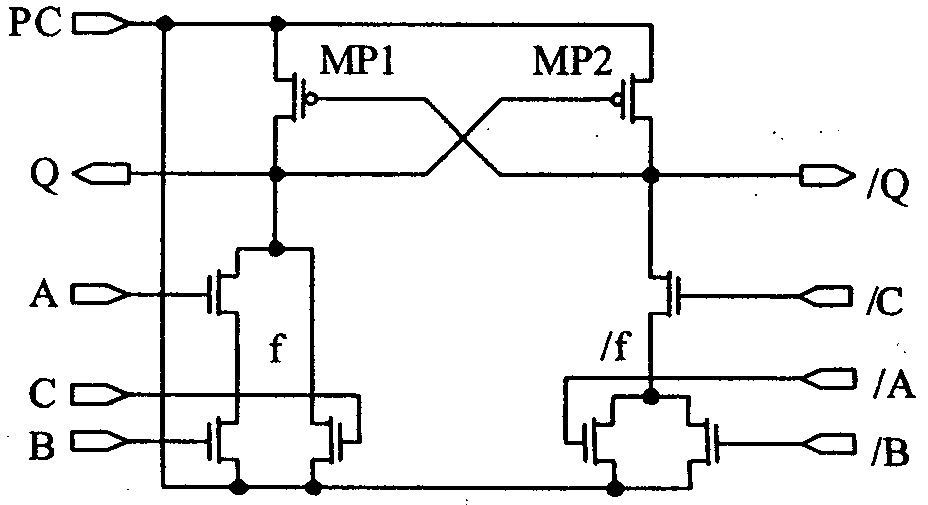
\includegraphics[width=\columnwidth]{../../images/palandor.png}
	\caption{A PAL AND-OR gate ($Q=A.B+C$) showing how to increase the complexity of the circuit \cite{PAL}}
	\label{fig:palandor}
\end{figure}


\subsubsection{LPAL}
\label{sec:LPAL}
Latched Pass-transistor Adiabatic Logic is a variation on PAL which adds transistors to disconnect the gate from the power clock.
These transistors can be seen in figure \ref{fig:lpal}, labelled as \emph{MN3} and \emph{MP3}.

\begin{figure}
	\centering
	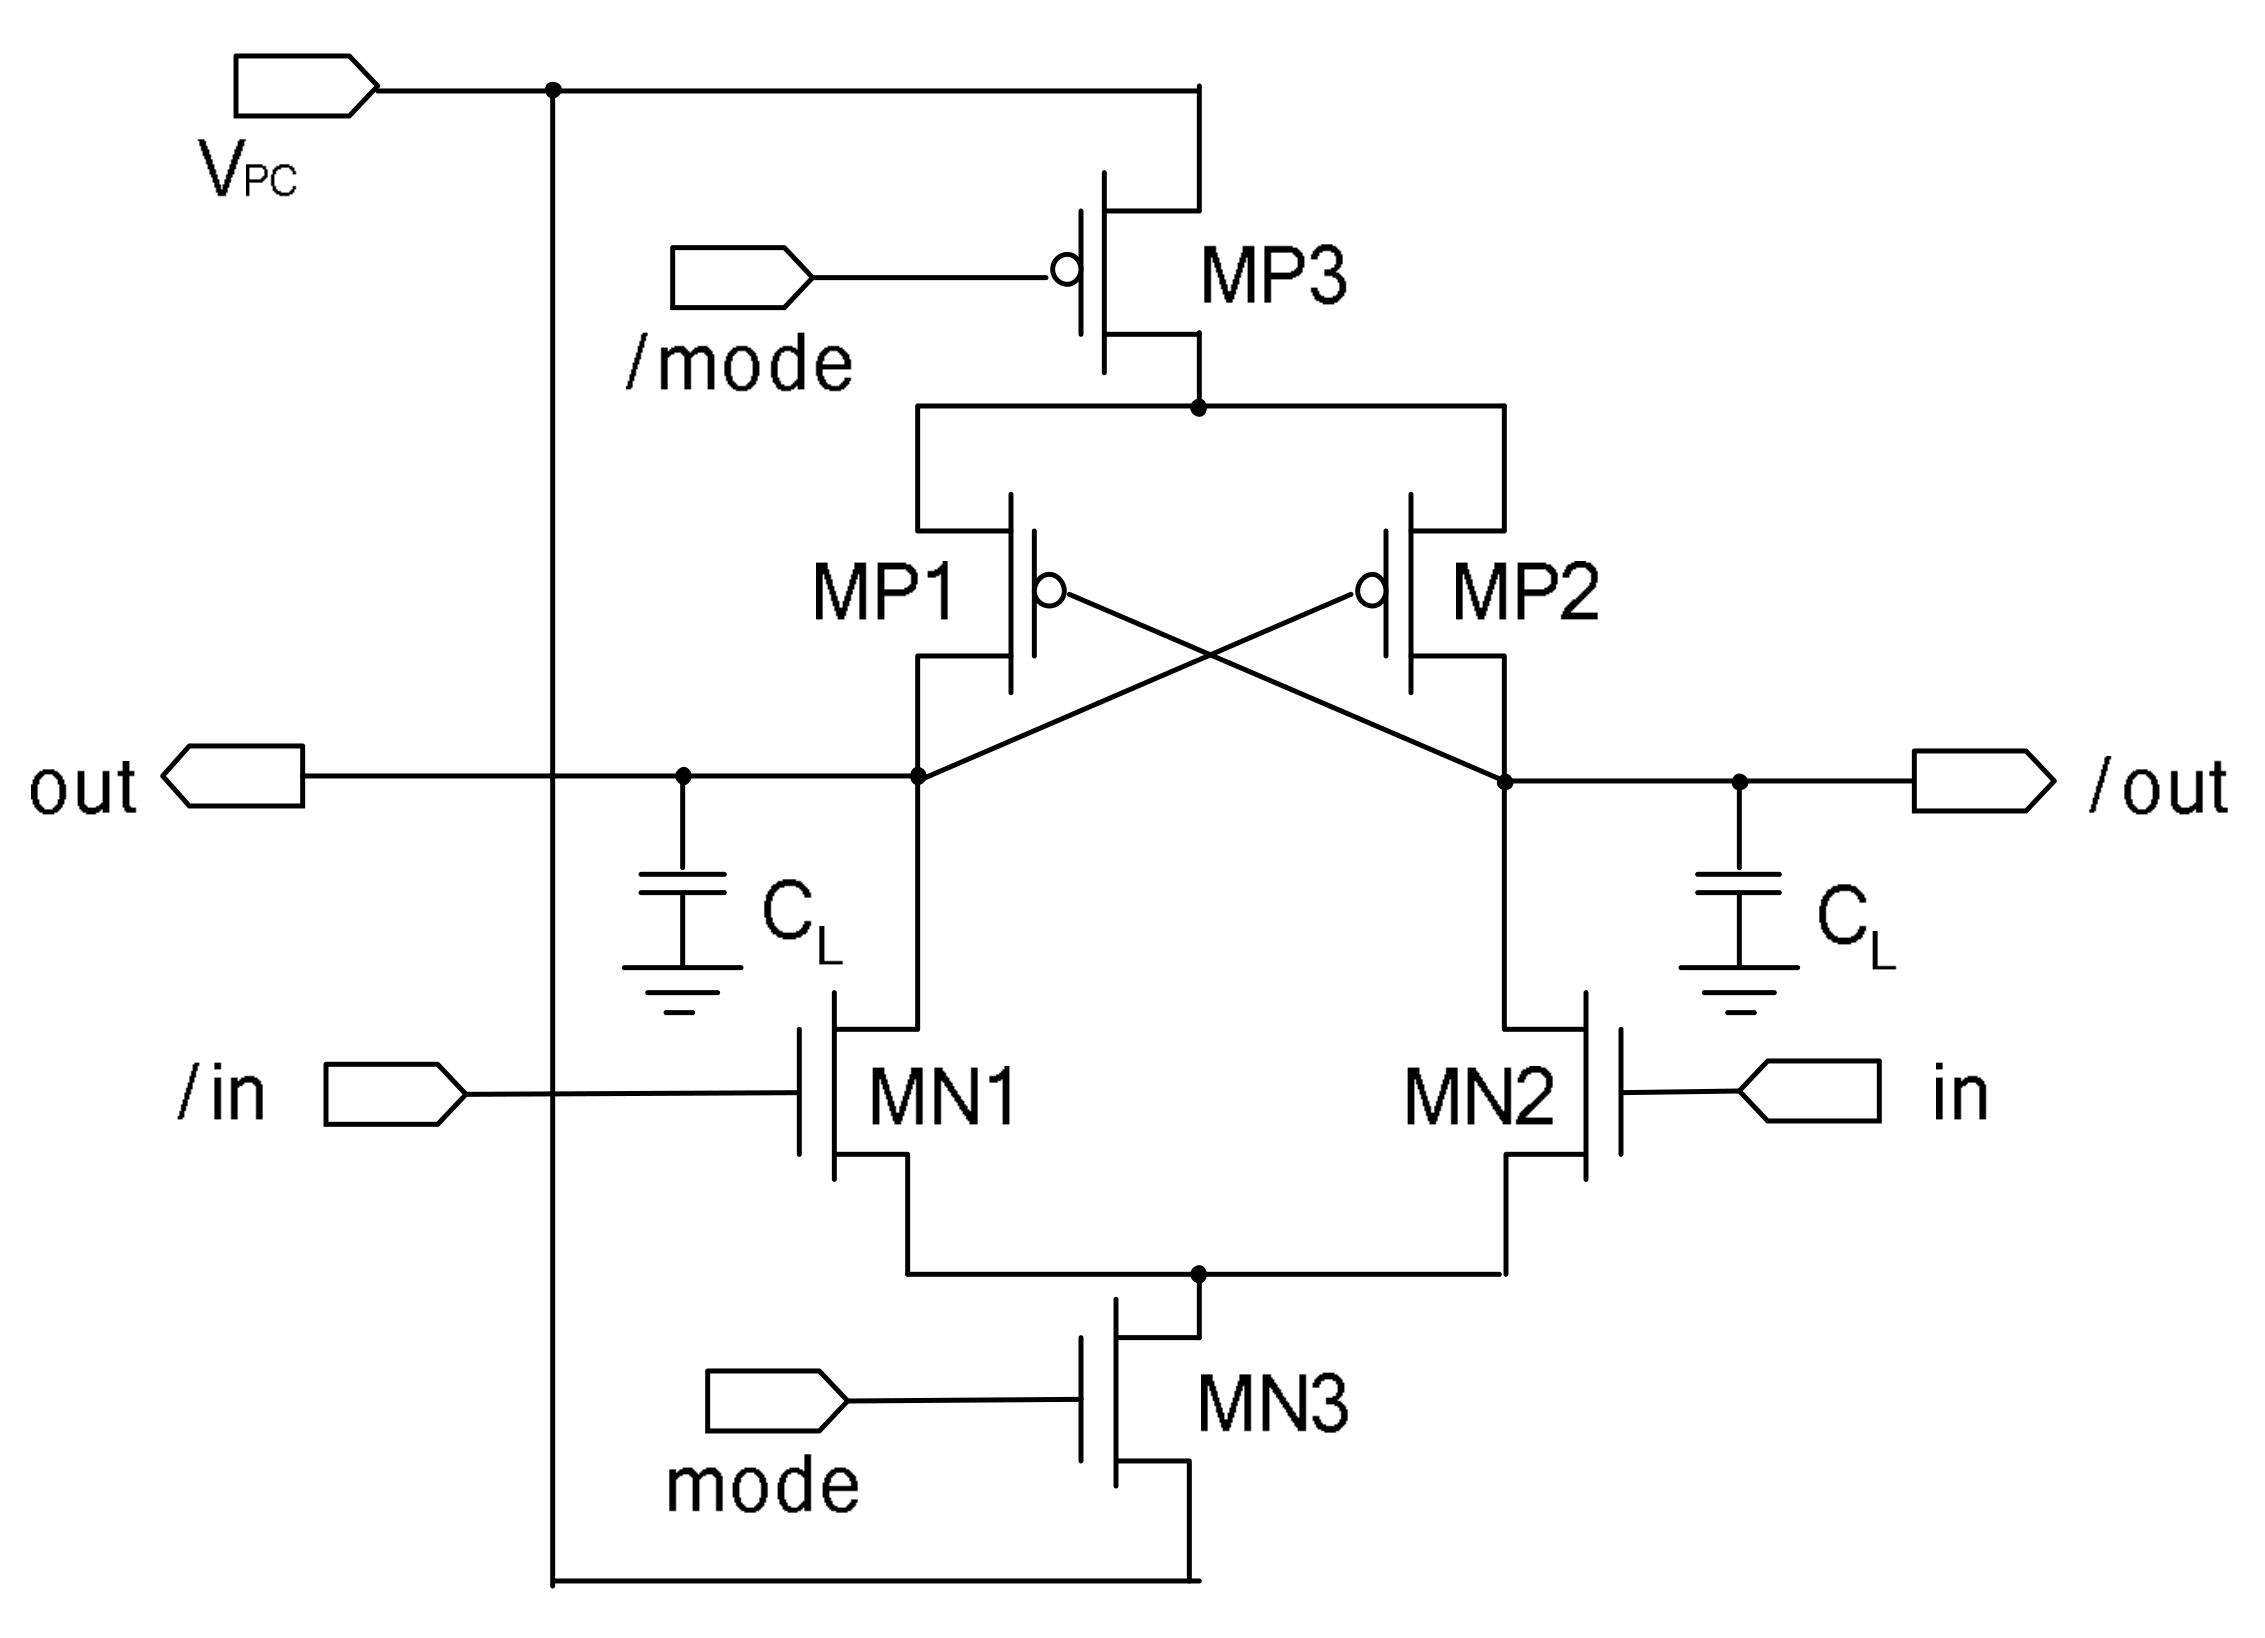
\includegraphics[width=\columnwidth]{../../images/LPAL.png}
	\caption{Circuit diagram of a LPAL inverter \cite{LPAL}}
	\label{fig:lpal}
\end{figure}

